\begin{itemize}
\item Ahmad Syafrizal Huda (1164062)
\item Annisa Fathoroni (1164067)
\item Puad Hamdani (1164084)
\item Rahmi Roza (1164085)
\item Tasya Wiendhyra (1164086)
\end{itemize}

\section{Definisi Flask GET}
Flask merupakan microframework yang dibangun dengan menggunakan bahasa pemrograman Python. Flask digunakan untuk me-develop sebuah aplikasi web. Flask merupakan microframework yang artinya flask membuat sebuah pengerjaan aplikasi web menjadi mudah dan simple karena dapat menjalankan sebuah web hanya dengan menggunakan 1 file Python. Flask membuat susunan kerja yang ringan, dan mudah tetapi juga dapat dikembangkan dengan mudah. Setiap data memiliki akses dengan berbagai HTTP Method seperti GET (Menerima data dalam bentuk array atau object) \cite{gunawan2018aplikasi}.
\subsection{pengertian GET request pada Flask}
GET request merupakan cara termundah untuk mengambil data dari pengguna. GET request tidak boleh mengubah status server yang dapat mengakibatkan efek samping.  Maka dari itu pengguna harus dapat membuat request yang sama dan harus mendapatkan hasil yang sama juga secara berkala. Oleh karena itu, GET request sangat ideal untuk memungkinkan pengguna untuk membedakan atau menentukan publikasi mana untuk dilihat\cite{dwyer2016flask}.
\subsection{Metode Flask GET}
Metode penyediaan perintah operasional untuk program  yang dikirimkan menggunakan protokol HTTP termasuk menyimpan program  di server; menghasilkan data meta di server, di mana data meta mencakup tabel pemetaan yang menghubungkan rentang waktu untuk program  ke rentang byte untuk program  mentransmisikan data meta dan tabel pemetaan ke klien yang terkait dengan server, menghasilkan dan mentransmisikan perintah GET HTTP dari klien  ke server sebagai fungsi dari perintah operasional yang diinginkan; dan memilih I-frame yang tepat di server dan mengirimkan I-frame ke klien sebagai tanggapan atas perintah HTTP GET \cite{xu2006method}.

\section{Implementasi Pada Flask GET}
\subsection{Sistem Terintegrasi Berbasis Ajax untuk Pengelolaan Data Bencana Alam di Indonesia}
Metode GET dan POST merupakan objek XHR yang sama bekerja sebagai standar HTTP request. Menggunakan salah satu, baik metode GET atau POST dapat digunakan untuk melakukan permintaan data dan menerima tanggapan dari server dengan format standar. Format standar yang dapat diterima dari server adalah XML, JSON (Javascript Object Notation), dan teks \cite{prasetyo2007sistem}.
\subsection{Sistem Terintegrasi Berbasis Ajax untuk Pengelolaan Data Bencana Alam di Indonesia}
Objek XHR (XMLHttpRequest) adalah inti dari Ajax angine. XHR merupakan objek yang memberikan kemampuan sebuah halaman untuk mendapatkan data (menggunakan metode GET) atau mengirim data (menggunakan metode POST) dari server yang prosesnya terjadi di belakang layar, itu berarti refresh browser tidak diperlukan sepanjang proses ini. Hal inilah yang menjadi factor kunci dalam memberikan kelebihan aplikasi kepada user. User tidak perlu mengetahui proses sehingga dapat focus dengan pekerjaan yang dilakukan \cite{prasetyo2007sistem}.
\subsection{Implementasi pengkodean sistem Python dengan versi 2.7.13.}
Implementasi pengkodean sistem, menggunakan Bahasa pemrograman Python dengan versi 2.7.13. Framework yang digunakan untuk sistem ini adalah Flask Micro-Framework. Adapun beberapa library yang mendukung sistem ini adalah:
\begin{enumerate}
\item Pandas
\item Matplotlib
\item Scikit-learn
\item Flask-CORS
\item Jupyter Notebook
\item Pymysql
\item Scipy
\end{enumerate}
Selain itu aplikasi juga dijalankan dalam server dan diatur oleh Apache Server dengan memanfaatkan mod wsgi. Database yang digunakan pada aplikasi ini adalah MySQL\cite{gunawan2018aplikasi}.

\section{Contoh Flask GET}
\subsection{Request sederhana pada Flask Framework}
Berikut ini merupakan contoh skrip dari GET request :
\begin{figure}[ht]
\centerline{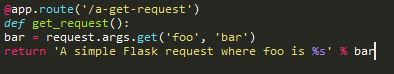
\includegraphics[width=1\textwidth]{figures/3FlaskGet.jpg}}
\caption{Method GET}
\label{labelgambar}
\end{figure}
Pada gambar\ref{labelgambar}Ini merupakan contoh sederhana dari apa GET request pada flask. Pada skrip ini hanya dilakukan pemeriksaan apakah query URL memiliki argumen yang disbut foo. apabila iya, maka akan menampilkan ini pada tanggapan, sedangkan jika tidak maka defaultnya adalah bar \cite{aggarwal2014flask}.

\section{Keamanan Flask GET}
\subsection{deteksi serangan dos dengan http get}
Serangan DoS ke layanan Web disebut serangan banjir http-get dan ancamannya meningkat dari hari ke hari. Dalam jenis serangan ini, klien jahat mengirim sejumlah besar permintaan http-get ke server Web target secara otomatis. Karena permintaan http-get ini memiliki format yang sah dan dikirim melalui koneksi TCP normal, intrusion detection system (IDS) tidak dapat mendeteksi mereka. Dalam tulisan ini, kami mengusulkan teknik pendeteksian pendeteksian http-get berdasarkan analisis perilaku akses halaman. Kami mengusulkan dua algoritme deteksi, yang satu berfokus pada urutan penelusuran laman dan yang lainnya berfokus pada korelasi dengan waktu penelusuran ke ukuran informasi laman. Kami menerapkan teknik deteksi dan mengevaluasi tingkat deteksi serangan, yaitu, false positive dan false negative. Hasilnya menunjukkan bahwa teknik kami dapat mendeteksi serangan banjir http-get secara efektif \cite{yatagai2007detection}.

\section{Pengertian Get Flask Pada Request}
\subsection{Mendapatkan masukan pengguna menggunakan HTTP GET}
Oleh karena itu, permintaan GET sangat ideal untuk memungkinkan pengguna kami menentukan publikasi mana untuk melihat. Mari kita memperluas proyek Headlines kami untuk menggabungkan memilih judul berdasarkan atas permintaan GET. Pertama, mari kita memodifikasi kode Python untuk melakukan hal berikut:
\begin{enumerate}
  \item Impor konteks permintaan dari Flask
  \item Hapus variabel URL dinamis
  \item Periksa untuk melihat apakah pengguna telah memasukkan publikasi yang valid sebagai argumen GET
  \item Lewati kueri pengguna dan publikasi ke templat
\end{enumerate}\cite{dwyer2016flask}.
 



